% This file was created with tikzplotlib v0.10.1.
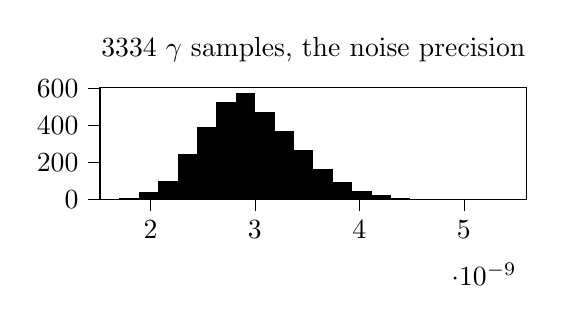
\begin{tikzpicture}

\definecolor{darkgray176}{RGB}{176,176,176}

\begin{axis}[
height=3cm,
tick align=outside,
tick pos=left,
title={3334 \(\displaystyle \gamma\) samples, the noise precision},
width=7cm,
x grid style={darkgray176},
xmin=1.51691907059514e-09, xmax=5.60137101243625e-09,
xtick style={color=black},
y grid style={darkgray176},
ymin=0, ymax=601.65,
ytick style={color=black}
]
\draw[draw=none,fill=black] (axis cs:1.70257597704247e-09,0) rectangle (axis cs:1.88823288348979e-09,8);
\draw[draw=none,fill=black] (axis cs:1.88823288348979e-09,0) rectangle (axis cs:2.07388978993711e-09,42);
\draw[draw=none,fill=black] (axis cs:2.07388978993711e-09,0) rectangle (axis cs:2.25954669638444e-09,101);
\draw[draw=none,fill=black] (axis cs:2.25954669638444e-09,0) rectangle (axis cs:2.44520360283176e-09,244);
\draw[draw=none,fill=black] (axis cs:2.44520360283176e-09,0) rectangle (axis cs:2.63086050927908e-09,389);
\draw[draw=none,fill=black] (axis cs:2.63086050927908e-09,0) rectangle (axis cs:2.8165174157264e-09,526);
\draw[draw=none,fill=black] (axis cs:2.8165174157264e-09,0) rectangle (axis cs:3.00217432217373e-09,573);
\draw[draw=none,fill=black] (axis cs:3.00217432217373e-09,0) rectangle (axis cs:3.18783122862105e-09,472);
\draw[draw=none,fill=black] (axis cs:3.18783122862105e-09,0) rectangle (axis cs:3.37348813506837e-09,371);
\draw[draw=none,fill=black] (axis cs:3.37348813506837e-09,0) rectangle (axis cs:3.5591450415157e-09,269);
\draw[draw=none,fill=black] (axis cs:3.5591450415157e-09,0) rectangle (axis cs:3.74480194796302e-09,162);
\draw[draw=none,fill=black] (axis cs:3.74480194796302e-09,0) rectangle (axis cs:3.93045885441034e-09,96);
\draw[draw=none,fill=black] (axis cs:3.93045885441034e-09,0) rectangle (axis cs:4.11611576085767e-09,45);
\draw[draw=none,fill=black] (axis cs:4.11611576085767e-09,0) rectangle (axis cs:4.30177266730499e-09,23);
\draw[draw=none,fill=black] (axis cs:4.30177266730499e-09,0) rectangle (axis cs:4.48742957375231e-09,7);
\draw[draw=none,fill=black] (axis cs:4.48742957375231e-09,0) rectangle (axis cs:4.67308648019964e-09,4);
\draw[draw=none,fill=black] (axis cs:4.67308648019964e-09,0) rectangle (axis cs:4.85874338664696e-09,0);
\draw[draw=none,fill=black] (axis cs:4.85874338664696e-09,0) rectangle (axis cs:5.04440029309428e-09,1);
\draw[draw=none,fill=black] (axis cs:5.04440029309428e-09,0) rectangle (axis cs:5.23005719954161e-09,0);
\draw[draw=none,fill=black] (axis cs:5.23005719954161e-09,0) rectangle (axis cs:5.41571410598893e-09,1);
\end{axis}

\end{tikzpicture}
